A threshold level is used to adjust the system for the current installation height of the camera. It sets a configuration parameter called lowestDistanceOverFloor. This is the limit of how short a person can be. The threshold should be set so that a "normal" person’s chest is not removed by the thresholding.

\begin{figure}[htb]
	\centering
	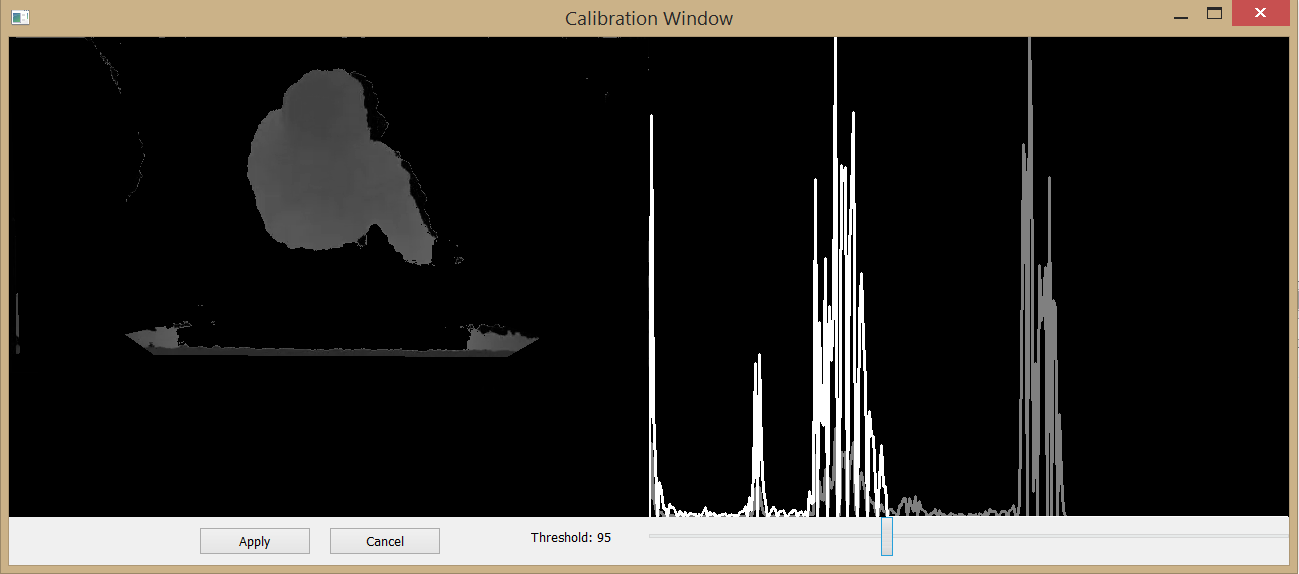
\includegraphics[width=\linewidth]{images/Calibration.png}
	\caption[Overview of the entire system]{\textit{Calibrating the lowestDistanceOverFloor threshold. A histogram i shown to help the user to se how much off different heights are present in the image. The selected heights are gray shaded.}}
	\label{fig:lowestDistanceOverFloor_calibration}  %Skapar referens till figuren
\end{figure}
